\index{numerical integration}
\index{quadrature}
\chapter{Numerical Integration I --- Quadrature Rules}
\newthought{Computing Integrals When Antiderivatives Don't Exist}


% ==============================================================================================
% INTRODUCTION BLOCK

\section{The Why}
\index{numerical integration!motivation}

\newthought{Many quantities we care about} are defined as integrals:
\begin{equation}
    I = \int_a^b f(x) \, dx
\end{equation}

In calculus, we learn the Fundamental Theorem: find an antiderivative $F(x)$ such that $F'(x) = f(x)$, then $I = F(b) - F(a)$. Clean, exact, elegant.

But here's the uncomfortable truth: \emph{most functions don't have nice closed-form antiderivatives}. The functions we encounter in practice---from physics, engineering, statistics, and machine learning---usually resist symbolic integration.

\newthought{Examples where analytical integration fails:}
\begin{itemize}
    \item $\int e^{-x^2} dx$ --- The Gaussian integral has no elementary antiderivative
    \item $\int \frac{\sin(x)}{x} dx$ --- The sine integral (Si function)
    \item $\int \sqrt{1 - k^2\sin^2(x)} dx$ --- Elliptic integrals
    \item $\int_\Omega p(x) \, dx$ where $p(x)$ is only known at sample points
\end{itemize}

\marginnote{\newthought{In machine learning:}
\begin{itemize}
    \item Expected loss: $\mathbb{E}[L] = \int L(x) p(x) dx$
    \item Bayesian posteriors
    \item Normalizing constants
    \item Marginal likelihoods
    \item Partition functions
\end{itemize}}

\newthought{In machine learning and artificial intelligence,} numerical integration appears constantly, often disguised:
\begin{itemize}
    \item \textbf{Batch averaging:} $\frac{1}{n}\sum_{i=1}^n L(x_i) \approx \int L(x) p(x) dx$ --- this IS numerical integration
    \item \textbf{Expected value computation:} Uncertainty quantification, risk assessment
    \item \textbf{Variational inference:} The ELBO involves intractable posterior integrals
    \item \textbf{Normalizing flows:} Change-of-variables with Jacobian determinants
    \item \textbf{Bayesian neural networks:} Marginalization over weight distributions
\end{itemize}

\newthought{Key insight:} Every time you compute a mini-batch mean in training, you're performing numerical integration. The batch average approximates the integral $\int L(\theta, x) p(x) dx$ over the data distribution.



\newpage
\subsection{Hands On Experience}
\index{numerical integration!hands-on}

\newthought{Consider computing} $\int_0^1 e^x \, dx$.

\textbf{Analytically:} This one we \emph{can} solve: $\int_0^1 e^x dx = [e^x]_0^1 = e - 1 \approx 1.71828$.

Let's pretend we can't, and approximate numerically.

\vspace{1em}
\textbf{Method 1: Rectangles (Midpoint Rule) with 2 intervals:}
\begin{align*}
    h &= \frac{1-0}{2} = 0.5 \\
    \text{Midpoints:} \quad x_1 &= 0.25, \quad x_2 = 0.75 \\
    I_{\text{mid}} &\approx h \cdot [f(0.25) + f(0.75)] \\
    &= 0.5 \cdot [e^{0.25} + e^{0.75}] \\
    &= 0.5 \cdot [1.284 + 2.117] \\
    &= 1.701
\end{align*}

Error: $|1.71828 - 1.701| = 0.017$ (about 1\%).

\marginnote{\newthought{Midpoint vs endpoints:} The midpoint rule uses the ``average height'' of each interval, which often gives better results than left or right endpoint methods.}

\vspace{1em}
\textbf{Method 2: Trapezoids with 2 intervals:}
\begin{align*}
    h &= 0.5 \\
    I_{\text{trap}} &\approx \frac{h}{2}[f(0) + 2f(0.5) + f(1)] \\
    &= \frac{0.5}{2}[1 + 2 \cdot 1.649 + 2.718] \\
    &= 0.25 \cdot 7.016 \\
    &= 1.754
\end{align*}

Error: $|1.71828 - 1.754| = 0.036$ (about 2\%)---worse than midpoint for this function!

\vspace{1em}
\textbf{With 4 intervals (midpoint):}
\begin{align*}
    h &= 0.25, \quad \text{midpoints at } 0.125, 0.375, 0.625, 0.875 \\
    I &\approx 0.25 \cdot [e^{0.125} + e^{0.375} + e^{0.625} + e^{0.875}] \\
    &= 0.25 \cdot [1.133 + 1.455 + 1.868 + 2.399] \\
    &= 1.714
\end{align*}

Error: $|1.71828 - 1.714| = 0.004$ (about 0.2\%).

\marginnote{\newthought{Doubling the points} reduced error by $\sim 4\times$. This suggests $O(h^2)$ convergence---the error decreases as the square of the step size.}

\newthought{Pattern:} More evaluation points $\Rightarrow$ better accuracy. But how fast? And can we do better than simple rectangles or trapezoids?


\vspace{2em}
\newthought{The Learning Objectives} of this chapter aim at providing you with the abilities to:
\begin{itemize}
    \item Understand numerical integration as polynomial interpolation + exact integration
    \item Derive and apply the trapezoid rule with error analysis
    \item Understand the Newton-Cotes family (Trapezoid, Simpson's, higher orders)
    \item Apply composite rules for improved accuracy on large intervals
    \item Recognize that batch averaging in ML is numerical integration
    \item Choose appropriate quadrature methods for different problem types
\end{itemize}




% ==============================================================================================
% MAIN THEORY BLOCK

\newpage
\section{From Riemann to Trapezoid}
\index{Riemann sum!to trapezoid}

\subsection{Riemann Sums: Where It All Begins}
\index{Riemann sum}

\newthought{The definition of the integral} comes from Riemann sums. This is how we \emph{define} what $\int_a^b f(x)\,dx$ means:
\begin{equation}
    \int_a^b f(x) \, dx = \lim_{n \to \infty} \sum_{i=0}^{n-1} f(x_i^*) \cdot h
\end{equation}

where $h = (b-a)/n$ is the width of each subinterval and $x_i^* \in [x_i, x_{i+1}]$ is some point in the $i$-th subinterval.

\marginnote{\newthought{Geometric interpretation:} We're approximating the area under the curve with $n$ thin rectangles. As $n \to \infty$, the approximation becomes exact.}

\newthought{Choices for sample point $x_i^*$:}
\begin{itemize}
    \item \textbf{Left endpoint:} $x_i^* = x_i = a + ih$
    \item \textbf{Right endpoint:} $x_i^* = x_{i+1} = a + (i+1)h$
    \item \textbf{Midpoint:} $x_i^* = a + (i + 0.5)h$
\end{itemize}

\begin{figure}[h]
    \centering
    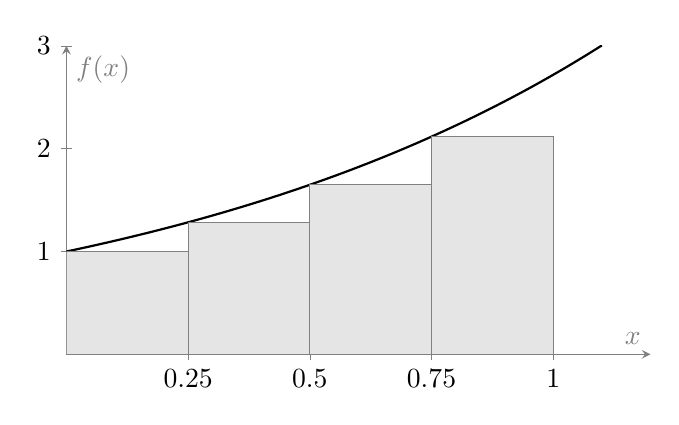
\begin{tikzpicture}
        \begin{axis}[
            width=9cm,
            height=5.5cm,
            axis x line=middle,
            axis y line=middle,
            xlabel={$x$},
            ylabel={$f(x)$},
            xmin=0, xmax=1.2,
            ymin=0, ymax=3,
            tick style={gray},
            label style={gray},
            axis line style={gray},
            xtick={0, 0.25, 0.5, 0.75, 1},
        ]
        % Function
        \addplot[black, thick, smooth, domain=0:1.1, samples=50] {exp(x)};
        % Left rectangles
        \addplot[fill=gray!20, draw=gray] coordinates {(0, 0) (0, 1) (0.25, 1) (0.25, 0)};
        \addplot[fill=gray!20, draw=gray] coordinates {(0.25, 0) (0.25, 1.284) (0.5, 1.284) (0.5, 0)};
        \addplot[fill=gray!20, draw=gray] coordinates {(0.5, 0) (0.5, 1.649) (0.75, 1.649) (0.75, 0)};
        \addplot[fill=gray!20, draw=gray] coordinates {(0.75, 0) (0.75, 2.117) (1, 2.117) (1, 0)};
        \end{axis}
    \end{tikzpicture}
    \caption{Left Riemann sum: rectangles use left endpoint height. For increasing functions like $e^x$, this systematically underestimates the integral.}
    \label{fig:left_riemann}
\end{figure}

\newthought{Error of Riemann sums:}
\begin{itemize}
    \item Left/Right endpoint: Error $O(h)$ --- first order
    \item Midpoint: Error $O(h^2)$ --- second order (surprisingly good!)
\end{itemize}

The midpoint rule achieves second-order accuracy because errors on the left and right halves of each interval tend to cancel.


\subsection{The Trapezoid Rule: Linear Interpolation}
\index{trapezoid rule}

\newthought{Key idea:} Instead of flat-topped rectangles, connect the function values with straight lines to form trapezoids.

\begin{figure}[h]
    \centering
    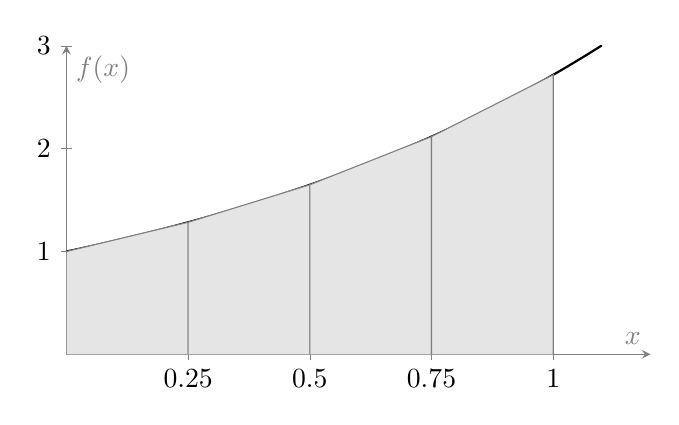
\begin{tikzpicture}
        \begin{axis}[
            width=9cm,
            height=5.5cm,
            axis x line=middle,
            axis y line=middle,
            xlabel={$x$},
            ylabel={$f(x)$},
            xmin=0, xmax=1.2,
            ymin=0, ymax=3,
            tick style={gray},
            label style={gray},
            axis line style={gray},
            xtick={0, 0.25, 0.5, 0.75, 1},
        ]
        % Function
        \addplot[black, thick, smooth, domain=0:1.1, samples=50] {exp(x)};
        % Trapezoids
        \addplot[fill=gray!20, draw=gray] coordinates {(0, 0) (0, 1) (0.25, 1.284) (0.25, 0)};
        \addplot[fill=gray!20, draw=gray] coordinates {(0.25, 0) (0.25, 1.284) (0.5, 1.649) (0.5, 0)};
        \addplot[fill=gray!20, draw=gray] coordinates {(0.5, 0) (0.5, 1.649) (0.75, 2.117) (0.75, 0)};
        \addplot[fill=gray!20, draw=gray] coordinates {(0.75, 0) (0.75, 2.117) (1, 2.718) (1, 0)};
        \end{axis}
    \end{tikzpicture}
    \caption{Trapezoid rule: linear interpolation between function values. The slanted tops follow the function more closely than flat rectangles.}
    \label{fig:trapezoid}
\end{figure}

\newthought{The trapezoid rule for $n$ subintervals:}
\begin{equation}
    \boxed{\int_a^b f(x) \, dx \approx T_n = \frac{h}{2}\left[f(a) + 2\sum_{i=1}^{n-1} f(x_i) + f(b)\right]}
\end{equation}

where $x_i = a + ih$ and $h = (b-a)/n$.

\marginnote{\newthought{Why the pattern 1-2-2-...-2-1?}
The area of one trapezoid is $\frac{h}{2}(f_i + f_{i+1})$. When we sum adjacent trapezoids, interior points get counted twice: once as a right endpoint, once as a left endpoint.}

\newthought{For a single interval $[a,b]$:}
\begin{equation}
    \int_a^b f(x) \, dx \approx \frac{b-a}{2}[f(a) + f(b)]
\end{equation}

This is just the area of one trapezoid with parallel sides $f(a)$ and $f(b)$, width $b-a$.

\begin{algorithm}[H]
\caption{Composite Trapezoid Rule}
\begin{algorithmic}[1]
    \Require Function $f$, interval $[a, b]$, number of subintervals $n$
    \State Compute step size: $h \gets (b - a) / n$
    \State Initialize sum: $S \gets f(a) + f(b)$
    \For{$i = 1$ to $n-1$}
        \State $x_i \gets a + i \cdot h$
        \State $S \gets S + 2 \cdot f(x_i)$
    \EndFor
    \State Compute integral: $I \gets h \cdot S / 2$
    \Return $I$
\end{algorithmic}
\end{algorithm}




\newpage
\section{Error Analysis}
\index{quadrature error}

\newthought{How accurate is the trapezoid rule?} We need to understand the error to choose step sizes wisely.

\subsection{Local Truncation Error}
\index{truncation error!local}

\newthought{Consider one interval} $[x_i, x_{i+1}]$ of width $h$.

The trapezoid approximation is the integral of the linear interpolant. Using Taylor expansion around the midpoint $x_i + h/2$:
\begin{equation}
    f(x) = f(m) + f'(m)(x-m) + \frac{f''(m)}{2}(x-m)^2 + O(h^3)
\end{equation}

After careful integration and comparison:
\begin{equation}
    \boxed{E_{\text{local}} = \int_{x_i}^{x_{i+1}} f(x)\,dx - \frac{h}{2}[f(x_i) + f(x_{i+1})] = -\frac{h^3}{12} f''(\xi)}
\end{equation}

for some $\xi \in [x_i, x_{i+1}]$.

\marginnote{\newthought{The error depends on $f''$:} The trapezoid rule is exact for linear functions ($f'' = 0$). For curves with larger curvature (larger $|f''|$), the error is larger.}


\subsection{Global Error}
\index{truncation error!global}

\newthought{With $n$ subintervals,} we sum $n$ local errors:
\begin{align}
    E_{\text{global}} &= \sum_{i=0}^{n-1} \left(-\frac{h^3}{12} f''(\xi_i)\right) \\
    &= -\frac{nh^3}{12} \bar{f''} \nonumber \\
    &= -\frac{(b-a)h^2}{12} f''(\xi) \nonumber
\end{align}

for some $\xi \in [a,b]$, using the generalized mean value theorem.

\begin{equation}
    \boxed{E_{\text{global}} = O(h^2)}
\end{equation}

\newthought{Practical implication:} Halving $h$ (doubling $n$) reduces error by factor of 4.


\subsection{Comparison of Methods}
\index{quadrature!method comparison}

\begin{table*}[ht]
\centering
\begin{tabular}{p{0.18\textwidth}p{0.15\textwidth}p{0.15\textwidth}p{0.30\textwidth}}
\toprule
\textbf{Method} & \textbf{Local Error} & \textbf{Global Error} & \textbf{Notes} \\
\midrule
Left/Right Riemann & $O(h^2)$ & $O(h)$ & Systematic bias \\
Midpoint & $O(h^3)$ & $O(h^2)$ & Errors cancel \\
Trapezoid & $O(h^3)$ & $O(h^2)$ & Easy to implement \\
Simpson's 1/3 & $O(h^5)$ & $O(h^4)$ & Quadratic fit \\
Simpson's 3/8 & $O(h^5)$ & $O(h^4)$ & Cubic fit \\
\bottomrule
\end{tabular}
\vspace{2em}
\caption{Comparison of quadrature method accuracies. Higher-order methods achieve given accuracy with fewer function evaluations.}
\label{tab:quadrature_comparison}
\end{table*}

\marginnote{\newthought{Order vs.\ work:} Higher-order methods achieve given accuracy with fewer function evaluations---but only for smooth functions. For discontinuous or noisy data, low-order methods may be more robust.}


\subsection{Numerical Verification}
\index{convergence verification}

For $\int_0^1 e^x dx = e - 1 \approx 1.71828$:

\begin{table*}[ht]
\centering
\begin{tabular}{p{0.08\textwidth}p{0.10\textwidth}p{0.22\textwidth}p{0.20\textwidth}p{0.10\textwidth}}
\toprule
$n$ & $h$ & Trapezoid Result & Error & Ratio \\
\midrule
2 & 0.5 & 1.7539 & $3.56 \times 10^{-2}$ & --- \\
4 & 0.25 & 1.7272 & $8.9 \times 10^{-3}$ & 4.0 \\
8 & 0.125 & 1.7205 & $2.2 \times 10^{-3}$ & 4.0 \\
16 & 0.0625 & 1.7188 & $5.6 \times 10^{-4}$ & 4.0 \\
32 & 0.03125 & 1.7184 & $1.4 \times 10^{-4}$ & 4.0 \\
\bottomrule
\end{tabular}
\vspace{2em}
\caption{Trapezoid rule convergence for $\int_0^1 e^x dx$. Each doubling of $n$ reduces error by factor 4, confirming $O(h^2)$.}
\label{tab:trapezoid_convergence}
\end{table*}

Each doubling of $n$ reduces error by exactly $4\times$, confirming $O(h^2)$ convergence.




\newpage
\section{Newton-Cotes Formulas}
\index{Newton-Cotes}

\newthought{The unifying idea:} Fit a polynomial through the function values and integrate the polynomial exactly.

\newthought{General procedure:}
\begin{enumerate}
    \item Choose $n+1$ equally spaced points $x_0, x_1, \ldots, x_n$ in $[a,b]$
    \item Construct the unique polynomial $P_n(x)$ of degree $\leq n$ passing through all points
    \item Integrate exactly: $\int_a^b f(x)\,dx \approx \int_a^b P_n(x)\,dx$
\end{enumerate}

The resulting formulas have the form:
\begin{equation}
    \int_a^b f(x)\,dx \approx \sum_{i=0}^n w_i f(x_i)
\end{equation}

where the weights $w_i$ depend only on $n$ and the interval length, not on $f$.


\subsection{Trapezoid Rule (n=1)}
\index{trapezoid rule!Newton-Cotes}

Linear polynomial through 2 points. Weights: $\frac{h}{2}(1, 1)$.
\begin{equation}
    \int_a^b f(x) \, dx \approx \frac{h}{2}[f(a) + f(b)]
\end{equation}

Exact for polynomials of degree $\leq 1$. Error: $O(h^3)$ local, $O(h^2)$ global.


\subsection{Simpson's 1/3 Rule (n=2)}
\index{Simpson's rule}

\newthought{Quadratic polynomial through 3 points.} The midpoint $m = (a+b)/2$ and half-width $h = (b-a)/2$ give:

\begin{equation}
    \boxed{\int_a^b f(x) \, dx \approx \frac{h}{3}[f(a) + 4f(m) + f(b)]}
\end{equation}

\marginnote{\newthought{Why 1-4-1?} These weights come from integrating the Lagrange interpolation polynomial. The middle point gets more weight because the parabola curves toward it.}

Weights: $\frac{h}{3}(1, 4, 1)$.

\newthought{Remarkable fact:} Simpson's rule is exact not just for quadratics, but also for \textbf{cubics}! The error is $O(h^5)$ locally, $O(h^4)$ globally.

\begin{figure}[h]
    \centering
    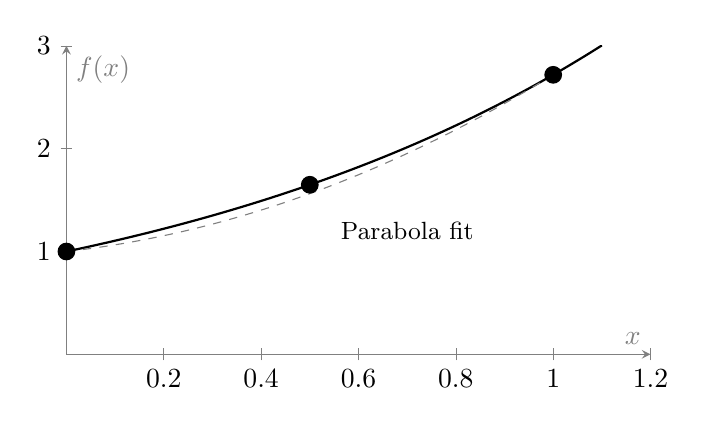
\begin{tikzpicture}
        \begin{axis}[
            width=9cm,
            height=5.5cm,
            axis x line=middle,
            axis y line=middle,
            xlabel={$x$},
            ylabel={$f(x)$},
            xmin=0, xmax=1.2,
            ymin=0, ymax=3,
            tick style={gray},
            label style={gray},
            axis line style={gray},
        ]
        % Function
        \addplot[black, thick, smooth, domain=0:1.1, samples=50] {exp(x)};
        % Quadratic fit
        \addplot[gray, dashed, smooth, domain=0:1, samples=50] {1 + 0.532*x + 1.186*x^2};
        % Points
        \addplot[black, only marks, mark=*, mark size=3pt] coordinates {(0, 1) (0.5, 1.649) (1, 2.718)};
        \node at (axis cs:0.7, 1.2) {\small Parabola fit};
        \end{axis}
    \end{tikzpicture}
    \caption{Simpson's rule: a parabola (dashed) through three points approximates the curve much better than a straight line.}
    \label{fig:simpson}
\end{figure}


\subsection{Simpson's 3/8 Rule (n=3)}
\index{Simpson's rule!3/8}

Cubic polynomial through 4 points:
\begin{equation}
    \int_a^b f(x) \, dx \approx \frac{3h}{8}[f_0 + 3f_1 + 3f_2 + f_3]
\end{equation}

where $h = (b-a)/3$. Weights: $\frac{3h}{8}(1, 3, 3, 1)$.

Also exact for cubics, same order as Simpson's 1/3.


\subsection{Higher-Order Newton-Cotes: A Warning}
\index{Newton-Cotes!instability}

\newthought{Why not use $n = 10$ or $n = 20$?}

For $n \geq 8$, Newton-Cotes formulas develop \textbf{negative weights}. This means:
\begin{itemize}
    \item Errors can amplify rather than cancel
    \item Results become unstable for noisy data
    \item The Runge phenomenon appears (recall interpolation chapter)
\end{itemize}

\marginnote{\newthought{Practical advice:} Stop at Simpson. For higher accuracy, use \emph{composite} rules (next section) or Gaussian quadrature (Chapter 9).}

This is the same issue we saw with polynomial interpolation: high-degree polynomials on equally-spaced points are unstable.




\newpage
\section{Composite Rules}
\index{composite rule}

\newthought{The problem:} Using one high-degree polynomial over the entire interval $[a,b]$ can be inaccurate for large intervals or oscillatory functions.

\newthought{The solution:} Apply low-order rules to many small subintervals, then sum the results. This is analogous to piecewise polynomial interpolation (splines).


\subsection{Composite Trapezoid Rule}
\index{trapezoid rule!composite}

Divide $[a,b]$ into $n$ subintervals, apply the trapezoid rule to each:

\begin{equation}
    \boxed{T_n = \frac{h}{2}\left[f(x_0) + 2\sum_{i=1}^{n-1} f(x_i) + f(x_n)\right]}
\end{equation}

where $h = (b-a)/n$ and $x_i = a + ih$.

\marginnote{\newthought{Pattern:} Endpoints get weight 1, interior points get weight 2 (they're shared between adjacent trapezoids).}

\textbf{Global error:} $O(h^2) = O(1/n^2)$. Doubling points quarters error.


\subsection{Composite Simpson's Rule}
\index{Simpson's rule!composite}

\marginnote{\newthought{Important:} $n$ must be \textbf{even} for composite Simpson, since each Simpson application uses 3 points spanning 2 subintervals.}

Divide $[a,b]$ into $n$ subintervals (with $n$ even), apply Simpson's 1/3 rule to pairs of subintervals:

\begin{equation}
    \boxed{S_n = \frac{h}{3}\left[f_0 + 4f_1 + 2f_2 + 4f_3 + 2f_4 + \cdots + 4f_{n-1} + f_n\right]}
\end{equation}

\textbf{Weight pattern:} 1, 4, 2, 4, 2, 4, 2, ..., 4, 2, 4, 1.

\textbf{Global error:} $O(h^4)$. Doubling points reduces error by factor of 16!

\begin{algorithm}[H]
\caption{Composite Simpson's Rule}
\begin{algorithmic}[1]
    \Require Function $f$, interval $[a, b]$, number of subintervals $n$ (must be even)
    \State Compute step size: $h \gets (b - a) / n$
    \State Initialize: $S \gets f(a) + f(b)$
    \For{$i = 1$ to $n-1$}
        \State $x_i \gets a + i \cdot h$
        \If{$i$ is odd}
            \State $S \gets S + 4 \cdot f(x_i)$
        \Else
            \State $S \gets S + 2 \cdot f(x_i)$
        \EndIf
    \EndFor
    \State Compute integral: $I \gets h \cdot S / 3$
    \Return $I$
\end{algorithmic}
\end{algorithm}


\subsection{Dramatic Comparison}
\index{quadrature!accuracy comparison}

For $\int_0^1 e^x dx = e - 1 \approx 1.71828$:

\begin{table*}[ht]
\centering
\begin{tabular}{p{0.08\textwidth}p{0.20\textwidth}p{0.20\textwidth}p{0.20\textwidth}}
\toprule
$n$ & Trap.\ Error & Simpson Error & Ratio \\
\midrule
4 & $8.9 \times 10^{-3}$ & $8.5 \times 10^{-6}$ & 1000$\times$ \\
8 & $2.2 \times 10^{-3}$ & $5.2 \times 10^{-7}$ & 4000$\times$ \\
16 & $5.6 \times 10^{-4}$ & $3.2 \times 10^{-8}$ & 17000$\times$ \\
32 & $1.4 \times 10^{-4}$ & $2.0 \times 10^{-9}$ & 70000$\times$ \\
\bottomrule
\end{tabular}
\vspace{2em}
\caption{Simpson's rule vs.\ trapezoid rule for $\int_0^1 e^x dx$. Simpson achieves dramatically higher accuracy for smooth functions.}
\label{tab:simpson_vs_trapezoid}
\end{table*}

\marginnote{\newthought{Simpson is remarkably efficient.} For smooth functions, it achieves near machine precision with relatively few points.}

For the same number of function evaluations, Simpson can be \emph{thousands of times} more accurate than the trapezoid rule!


\subsection{When Composite Simpson Fails}
\index{Simpson's rule!limitations}

\newthought{Caution:} Simpson's superiority depends on smoothness.

\begin{itemize}
    \item \textbf{Discontinuous $f$:} Polynomial interpolation across a jump is terrible. Use trapezoid (or break the interval at discontinuities).
    \item \textbf{Noisy data:} High-order methods amplify noise. Trapezoid is more robust.
    \item \textbf{Non-smooth derivatives:} If $f'''$ is discontinuous, Simpson's $O(h^4)$ may not be achieved.
\end{itemize}




% ==============================================================================================
% STUDENT ACTIVATION BLOCK

\newpage
\section{Examples \& Exercises}
\index{quadrature!exercises}

\marginnote{\newthought{Code} can be found at \url{https://github.com/Quillstacks/lecturecode_numericalmethods.git}.}

\newthought{Exercise 1: Trapezoid by hand.} Compute $\int_0^\pi \sin(x) dx$ using the composite trapezoid rule with $n = 2$ and $n = 4$.

The exact answer is $[-\cos(x)]_0^\pi = -(-1) - (-1) = 2$.

\vspace{0.5em}
\textit{Solution for $n=2$:}
\begin{align*}
    h &= \pi/2, \quad x_0 = 0, \quad x_1 = \pi/2, \quad x_2 = \pi \\
    T_2 &= \frac{\pi/2}{2}[\sin(0) + 2\sin(\pi/2) + \sin(\pi)] \\
    &= \frac{\pi}{4}[0 + 2 \cdot 1 + 0] = \frac{\pi}{2} \approx 1.571
\end{align*}
Error: $|2 - 1.571| = 0.429$ (21\%).

\vspace{0.5em}
\textit{Now try $n=4$:} You should get $T_4 \approx 1.896$, error $\approx 0.104$ (5\%).


\vspace{2em}
\newthought{Exercise 2: Simpson's rule.} Use Simpson's 1/3 rule to compute $\int_0^2 x^3 dx$ with a single application (3 points: 0, 1, 2).

\begin{enumerate}[label=(\alph*)]
    \item Apply the formula: $S = \frac{h}{3}[f(0) + 4f(1) + f(2)]$ with $h = 1$.
    \item Compare with exact value $[x^4/4]_0^2 = 4$.
    \item Explain why Simpson is exact for this cubic polynomial.
\end{enumerate}


\vspace{2em}
\newthought{Exercise 3: Error order verification.} For $\int_0^1 e^{-x^2} dx$ (no closed form!):
\begin{enumerate}[label=(\alph*)]
    \item Compute trapezoid approximations with $n = 10, 20, 40, 80$.
    \item Compute the ratios of successive errors: $E_{n}/E_{2n}$.
    \item Verify the ratios approach 4 (confirming $O(h^2)$ convergence).
    \item Repeat for Simpson and verify ratios approach 16.
\end{enumerate}


\vspace{2em}
\newthought{Exercise 4: Connection to Machine Learning.} The empirical loss is:
\begin{equation}
    L_{\text{emp}}(\theta) = \frac{1}{n}\sum_{i=1}^n \ell(\theta, x_i)
\end{equation}

This approximates the expected loss $L(\theta) = \int \ell(\theta, x) p(x) dx$.

\begin{enumerate}[label=(\alph*)]
    \item What quadrature rule is the batch mean equivalent to? (Hint: equal weights)
    \item If data points are uniformly distributed, what does this say about the sampling?
    \item How does importance sampling relate to non-uniform quadrature weights?
    \item Why might stratified sampling improve the integral estimate?
\end{enumerate}


\vspace{2em}
\newthought{Exercise 5: Choosing methods.} For each integral, recommend trapezoid or Simpson and justify:
\begin{enumerate}[label=(\alph*)]
    \item $\int_0^{10} \sin(x^2) dx$ (smooth, oscillatory)
    \item $\int_0^1 |x - 0.5| dx$ (V-shaped, non-smooth at $x = 0.5$)
    \item $\int_0^1 f(x) dx$ where $f$ is known only from noisy measurements
\end{enumerate}




\newpage
\section{Self-Reflection and Recap}
\index{quadrature!recap}

\newthought{Self-Reflection} Questions to guide your understanding:
\begin{itemize}
    \item How does batch size in SGD relate to quadrature accuracy?
    \item What happens if $f$ has discontinuities? Does quadrature still work?
    \item Why not use degree-100 Newton-Cotes? (Hint: Runge phenomenon, negative weights)
    \item For the same number of function evaluations, when is Simpson better than trapezoid? When might trapezoid be preferred?
    \item How is the trapezoid rule related to linear interpolation?
    \item Why is the midpoint rule more accurate than left/right Riemann sums?
\end{itemize}


\newthought{Recap} of Key Concepts:
\begin{itemize}
    \item \textbf{Numerical integration} approximates $\int_a^b f(x)\,dx$ using weighted sums of function values.
    \item \textbf{Trapezoid rule:} Linear interpolation between points. Error $O(h^2)$.
    \item \textbf{Simpson's rule:} Quadratic interpolation. Error $O(h^4)$, exact for cubics.
    \item \textbf{Newton-Cotes formulas:} A family based on polynomial interpolation. Higher orders are unstable.
    \item \textbf{Composite rules:} Apply simple rules to many subintervals. The practical choice for accuracy.
    \item \textbf{ML connection:} Batch averaging $\frac{1}{n}\sum L(x_i)$ IS numerical integration over data distribution.
\end{itemize}


\marginnote[2em]{\newthought{Teaser.} To halve the error with trapezoid, we need $4\times$ more function evaluations. Can we get \textbf{more accuracy without more evaluations}? And what about high-dimensional integrals where the curse of dimensionality strikes?}

\newthought{Beyond fixed-order methods.} The trapezoid rule with $n$ points gives error $O(1/n^2)$. Simpson gives $O(1/n^4)$. Can we do better with the \emph{same} function values?

Remarkably, yes. Richardson extrapolation and Romberg integration extract higher-order accuracy by cleverly combining results at different step sizes---no new function evaluations required.

And for high-dimensional integrals, deterministic quadrature faces the \textbf{curse of dimensionality}: $N^d$ points in $d$ dimensions. Monte Carlo methods escape this curse with errors that scale as $O(1/\sqrt{N})$ regardless of dimension. The next chapter explores these powerful techniques.



%%%%%%%%%%%%%%%%%%%%%%%%%%%%%%%%%%%%%%%%%%%%%%%%%%%%%%%%%%%%%%%%%%%%%%%%%%%%%%
